\section*{Analysis}
\label{Analyse}
%
Based on the results presented in the previous section it is possible to analyse how well a fit the BTL and preference tree are.\blankline
%
The number of possible stocastic violations in the data is 20, and from theese one moderate and five strong stocastic violations was found. This combined with the Chi-square test, which calculated a p-value at 0.0055, showed that a BTL-model would not be a good fit. Instead a preference tree was made.\blankline
%
As mentioned different types of preference trees was testet, but only two preference trees had a p-value high enough to fit. Theese two preference trees is shown on \autoref{fig:Tree1overveiw} and \autoref{fig:Tree2overveiw}. From matlab the value for every line segment of the preference tree is calculated. This length of the line segment is presented in \autoref{tab:Length1} for the first preference tree and \autoref{tab:Length2} for the second preference tree.  

%
\begin{table}[H]
	\centering
	\begin{tabular}{@{}ll@{}}
		\toprule
		Number of line segment    & Length of line segment \\ \midrule
		1									      & 0.1976   \\
		2      									  & 0.0277   \\
		3      									  & 0.0376   \\
		4      									  & 0.0259   \\
		5      									  & 0.6931   \\
		6      									  & 0.0509   \\
		7      									  & 0.8717   \\
		8								          & 0.0727   \\ \bottomrule
	\end{tabular}
	\caption{The tabel shows every length of the line segments from the first preference tree.}
	\label{tab:Length1}
\end{table} 
\noindent 
% 
\begin{table}[H]
	\centering
	\begin{tabular}{@{}ll@{}}
		\toprule
		Number of line segment     & Length of line segment \\ \midrule
		1							      & $3.36\cdot10^{15}$   \\
		2      							  & $4.37\cdot10^{14}$   \\
		3      							  & $5.98\cdot10^{14}$   \\
		4      							  & $7.66\cdot10^{14}$   \\
		5      							  & $3.58\cdot10^{16}$   \\
		6     							  & $4.00\cdot10^{15}$   \\
		7      							  & $1.39\cdot10^{15}$   \\
		8						          & $9.69\cdot10^{15}$   \\
		9								  & $1.30\cdot10^{15}$   \\ \bottomrule
	\end{tabular}
	\caption{The tabel shows every length of the line segments from the second preference tree.}
	\label{tab:Length2}
\end{table} 
\noindent 
%
The scale values for every drug is calculated by adding all lengt leading from the drug up to the starting point and is presented in \autoref{tab:ScaleValues1} for the first preference tree and \autoref{tab:ScaleValues2} for the second preference tree.\blankline
% 
\begin{table}[H]
	\centering
	\begin{tabular}{@{}ll@{}}
		\toprule
		Drugs     & Scale value \\ \midrule
		Alcohol	  & 0.1976   \\
		Tobacco	  & 0.1004   \\
		Cannabis	  & 0.1103   \\
		Ecstasy	  & 0.9703   \\
		Heroin	  & 1.6376   \\
		Cocaine	  & 0.9953   \\	\bottomrule
	\end{tabular}
	\caption{The tabel shows the scale values of the different drugs for the first preference tree.}
	\label{tab:ScaleValues1}
\end{table} 
\noindent 
%

\begin{table}[H]
	\centering
	\begin{tabular}{@{}ll@{}}
		\toprule
		Drugs     & Scale value \\ \midrule
		Alcohol	  & $3.36\cdot10^{15}$   \\
		Tobacco	  & $1.74\cdot10^{15}$   \\
		Cannabis	  & $1.90\cdot10^{15}$   \\
		Ecstasy	  & $1.31\cdot10^{16}$   \\
		Heroin	  & $4.82\cdot10^{16}$   \\
		Cocaine	  & $1.50\cdot10^{16}$   \\	\bottomrule
	\end{tabular}
	\caption{The tabel shows the scale values of the different drugs for the second preference tree.}
	\label{tab:ScaleValues2}
\end{table} 
\noindent 
%
To illustrate how the different drugs are evaluated based on health risks \autoref{fig:Tree1real} for the first preference tree are drawn and labeled. \autoref{fig:Tree2real} shows the second preference tree drawn and labeled. 
%
\begin{figure}[H]
\centering
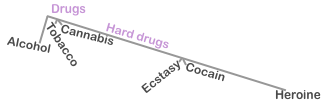
\includegraphics[width = 0.80\textwidth]{Figure/Tree1real}
\caption{The figure shows the real first preference tree with labels on the line segments.}
\label{fig:Tree1real}
\end{figure}
\noindent
%
\begin{figure}[H]
	\centering
	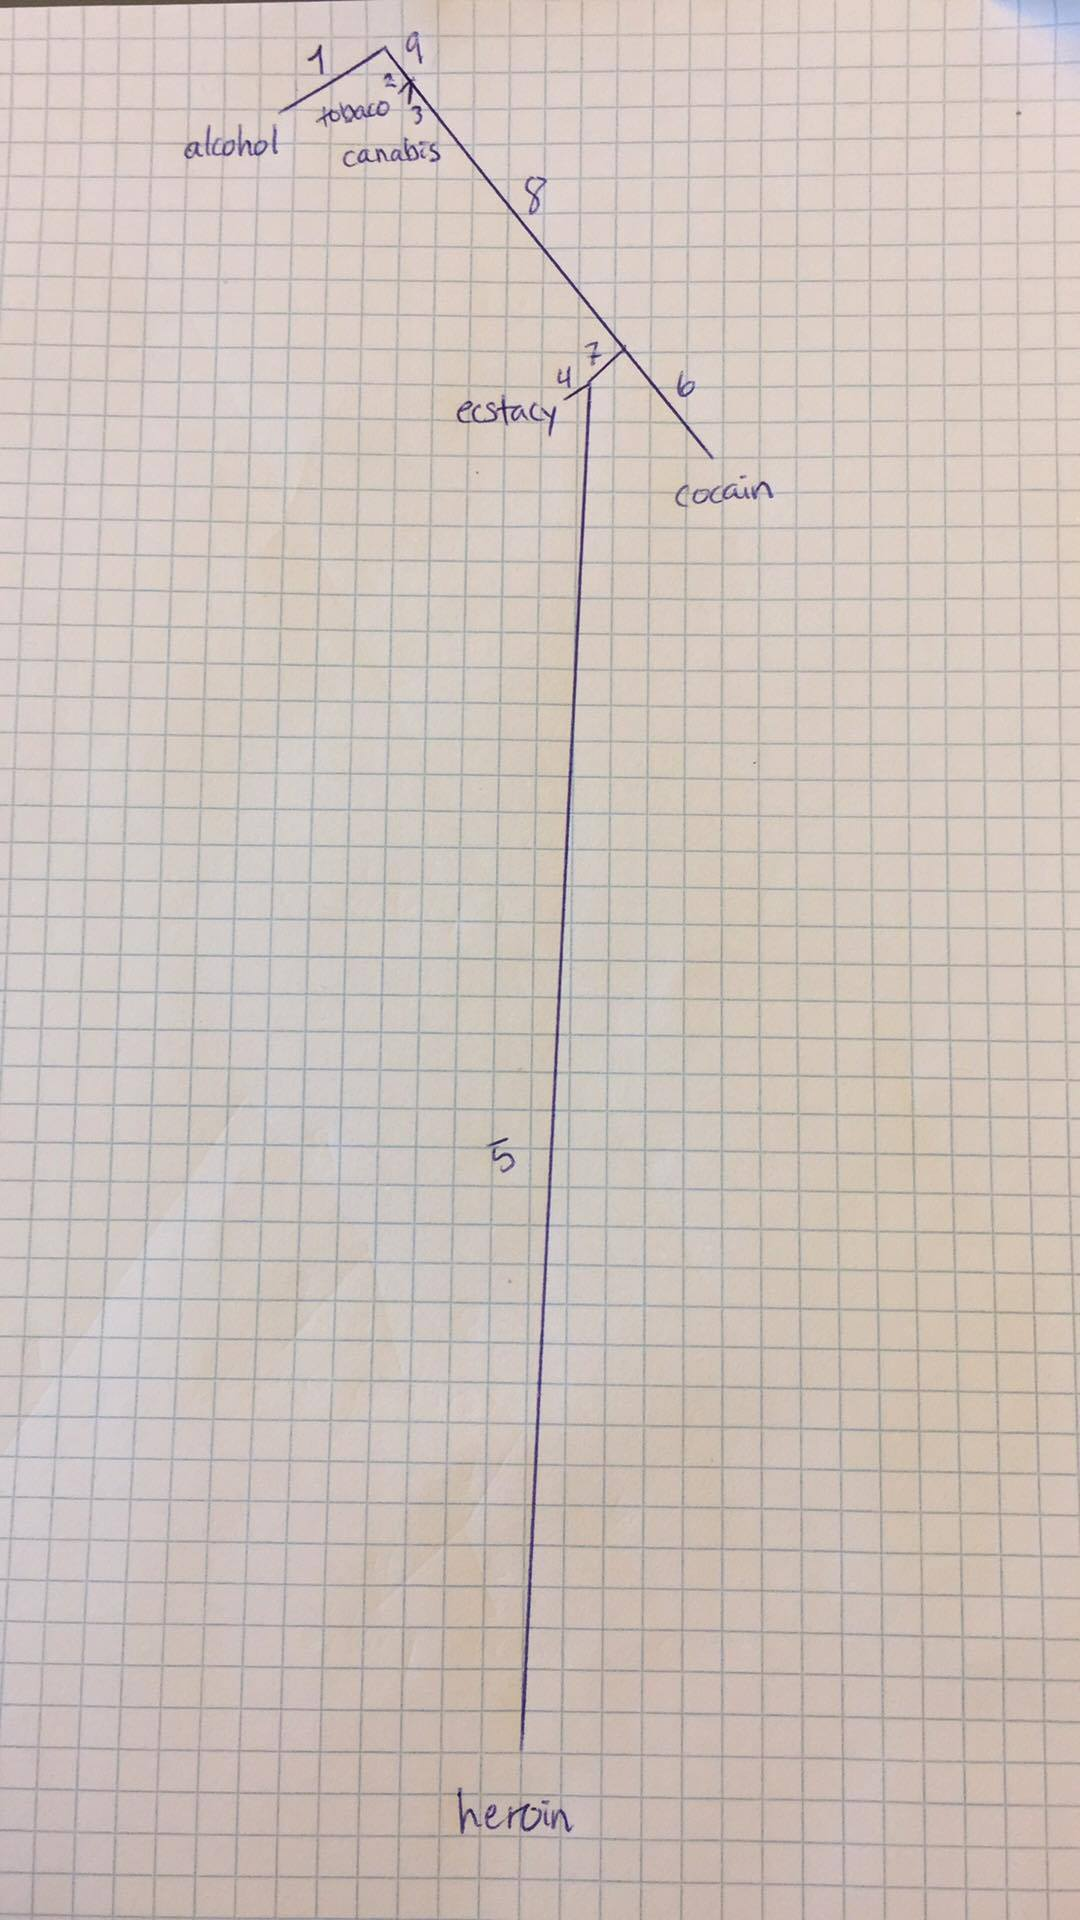
\includegraphics[width = 0.80\textwidth]{Figure/Tree2real}
	\caption{The figure shows the real second preference tree with labels on the line segments.}
	\label{fig:Tree2real}
\end{figure}
\noindent
%
%indsæt figurer af de tegnede preference trees her.
To signify what the analysis shows the scale values for each drug and their respective confidence interval are plottet in \autoref{fig:}.

%insæt confidensinterval og skriv noget om det 